\chapter{MATSim as a Monte-Carlo Engine}
\label{ch:montecarlo}
% ##################################################################################################################

\hfill \textbf{Author:} Gunnar Flötteröd

\begin{center} 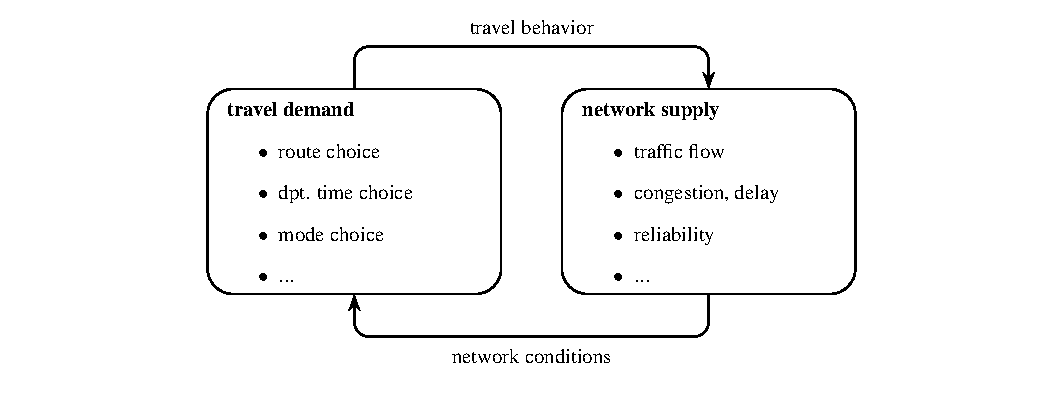
\includegraphics[width=0.7\textwidth, angle=0]{understanding/figures/mc/fig0.pdf} \end{center}

% ##################################################################################################################

\makeatletter

%%%%%%%%%%%%%%%%%%%%%%%%%%%%%% LyX specific LaTeX commands.
%% Because html converters don't know tabularnewline
\providecommand{\tabularnewline}{\\}
\floatstyle{ruled}
\newfloat{algorithm}{tbp}{loa}
\providecommand{\algorithmname}{Algorithm}
\floatname{algorithm}{\protect\algorithmname}

\makeatother

% ##################################################################################################################
\section{Introduction}

{}``Agents'' that {}``learn'' in a {}``synthetic reality'' is common language 
in Artificial Intelligence \citep{RusselNorvig2010ArtificialIntelligence} and/or 
Multi-Agent simulation~\citep{FerberBook}, but it does
not belong to the standard terminology of transport modeling. This
chapter phrases the functioning of MATSim in terms of modeling and simulation concepts
that are more established in the transportation field.
% \kai{Gunnar, habe an obigem Satz ein wenig gebastelt.  Wir haben uns diese Sprache 
% ja nicht selbst ausgedacht; sie war immer nur eine Reaktion auf Dinge, die wir 
% anderswo gelesen haben, und die u.E.\ besser passten als die etabliertere Terminologie.}

It is important to distinguish between a \gls{model} and a \gls{simulation}. A
model describes certain aspects of a system. A simulation evaluates
a model. For instance, a simple route choice model may state that
route A is selected with 25\% probability and route B with 75\% probability.
A simulation of this model then draws one or more realizations (route
choices) from this distribution. One always needs a model before one
can simulate. Possible feedbacks from simulation to modeling comprise
(i) new insights into emergent model properties and (ii) computational
constraints that prohibit overly complex model specifications. In
MATSim, both feedbacks are strong drivers of the modeling. 


% ----------
\createfigure%
{Demand/supply perspective on MATSim}%
{Demand/supply perspective on MATSim}%
{\label{fig:Demand/supply-perspective-on}}%
{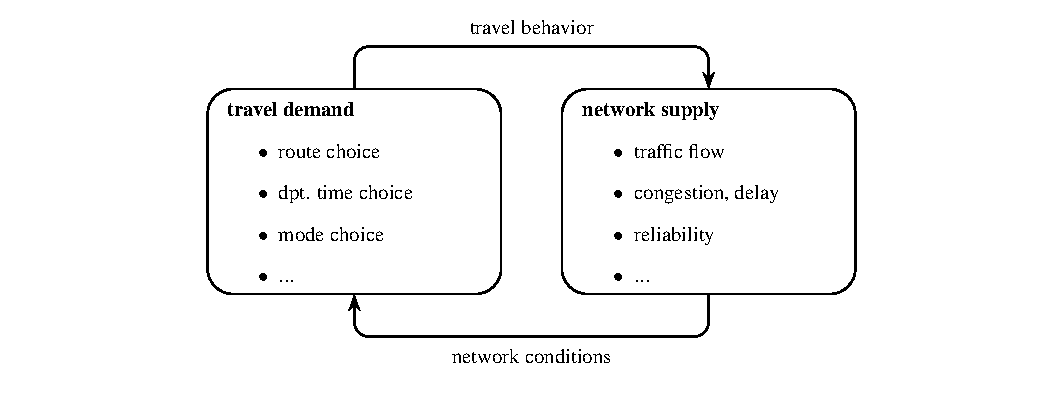
\includegraphics[width=0.99\textwidth, angle=0]{understanding/figures/mc/fig0.pdf}}%
{}
% ----------

Consider Figure~\ref{fig:Demand/supply-perspective-on}. It displays
MATSim as a model system comprising a (travel) demand model and a
(network) supply model. The travel demand model predicts the behavior
of travelers given their information about the network conditions.
The network supply model predicts these network conditions given a
certain travel behavior chosen by all travelers in the system. On
top of this comes the modeling assumption that demand and supply should
be mutually consistent, in the sense that the network conditions resulting
from a certain travel behavior are statistically equal to the network
conditions that caused this behavior.

Simulation addresses the question of how to identify this state of
mutual demand/supply consistency, i.e.\ it solves the model. The model
system shown in Figure~\ref{fig:Demand/supply-perspective-on} is
complicated -- it nonlinear, stochastic, and extremely high-dimensional.
The only known technique to solve it exploits an additional modeling
assumption that justifies the real occurrence of demand/supply consistency:
Travelers adjust their behavior for their own benefit, and they only
stop doing that when further improvement is insubstantial. Demand/supply
consistency characterizes the outcome of this process jointly for
all travelers.

\begin{algorithm}
\caption{\label{alg:Iterative-scheme-to}Iterative scheme to reach demand/supply
consistency}

\begin{enumerate}
\item Create a synthetic agent population.
\item Create a synthetic environment.
\item Iterate:

\begin{enumerate}
\item All agents chooses some planned travel behavior.
\item All agents execute their travel plans.
\item All agents see the resulting network conditions.\end{enumerate}
\end{enumerate}
\end{algorithm}


Now consider Algorithm~\ref{alg:Iterative-scheme-to}. It displays
the high-level simulation logic of MATSim. This is indeed a logic
that iteratively adjusts travel demand. If this logic adjusts the
simulated behavior of the simulated travelers until further simulated
improvements are insubstantial, then this logic may be expected to
approach a state of demand/supply consistency. That is, Algorithm~\ref{alg:Iterative-scheme-to}
may be a valid solution method for the model system shown in Figure~\ref{fig:Demand/supply-perspective-on}.
However, that model system does not specify how demand and supply
become consistent, it merely specifies that this eventually happens.
The only modeling assumption made is that some process of this type
exists. The purpose of Algorithm~\ref{alg:Iterative-scheme-to} is
not to mimic this (unspecified) process. It only identifies the final
outcome of that process.

The fact that Algorithm~\ref{alg:Iterative-scheme-to} looks like
a mimicry of real urban day-to-day dynamics invites misleading interpretations
of the underlying model system. In particular, it is a misconception
that the there is more than a superficial resemblance between the
{}``learning agents'' in MATSim and the (hardly understood) learning
processes of real humans. If the notion of {}``learning'' has to
be used at all when interpreting Algorithm~\ref{alg:Iterative-scheme-to},
it should be understood as {}``moving a MATSim model closer to its
solution point''.  Also see Sec.~\ref{sec:transients-vs-learning}.
% \kai{Gunnar, I hope that this is ok.}

The remainder of this chapter phrases these statements more technically and explains 
its implications for the interpretation of MATSim outputs.  This presentation is in parts a 
more technical reformulation of Chapter~\ref{ch:abta}.


\section{\label{sec:Relaxation-as-a}Relaxation as a Stochastic Process}


\subsection{\label{sub:Probabilistic-model-components}Probabilistic Model Components}

Algorithm~\ref{alg:Iterative-scheme-to} can be written more formally.
Denoting the iteration index by $k$, the following happens in every
iteration:
\begin{enumerate}
\item \label{enu:Every-traveler-chooses}All agents choose some planned
travel behavior, resulting in the travel demand $D^{k}$ of the entire
agent population.
\item \label{enu:All-travelers-execute}All agents execute their travel
plans, resulting in the (time-of-day dependent) network conditions
$S^{k}$.
\item \label{enu:All-travelers-observe}All agents see the resulting network
conditions $S^{k}$. As a result, the information $Z^{k}$ is now
available to the agents.
\end{enumerate}
The variables $D$ and $Z$ apply to the population as a whole, comprising
all agents. Similarly, the variable $S$ represents the network conditions
for an entire day and for the entire physical system. Given MATSim's
high level of detail, one hence may think of $D$, $S$ and $Z$ as
placeholders for arbitrarily large data and complex structures.
%\note{Refer to corresponding data containers in MATSim?}\kai{done, see next.}  
Under standard conditions, $D$ corresponds to the set of selected plans, 
$S$ corresponds to the collection of all events, 
and $Z$ corresponds to the full plans file including the scores.

Step~\ref{enu:Every-traveler-chooses} evaluates the (stochastic)
travel behavior model of each agent. Technically, this comprises (i)
an optional update of the plan choice set and (ii) the choice of one
plan to be executed. Symbolically, this is written as
\begin{equation}
D^{k}\sim P(D\mid Z^{k-1}),\label{eq:choice-model}
\end{equation}
meaning that the travel demand of iteration $k$ follows a probability
distribution that is conditional on the information $Z^{k-1}$ that
was available to the agents at the end of iteration $k-1$.

%% \kai{@Gunnar: Wir haben $S$ für score im Buch.  Habe daher aus Deinem $S$ mal $C$ gemacht; das entspricht auch der Notation in der Lehrveranstaltung Verkehrstelematik ($C$ $=$ ``conditions'').}
%% \gunnar{ok}

Step~\ref{enu:All-travelers-execute} runs the (stochastic) mobility
simulation that moves all agents jointly through the network. In symbols,
this becomes
\begin{equation}
C^{k}\sim P(S\mid D^{k}),\label{eq:network-loading-model}
\end{equation}
meaning that the network conditions of iteration $k$ follows a probability
distribution that is conditional on the demand $D^{k}$. 

Step~\ref{enu:All-travelers-observe} updates (possibly in a stochastic
way) the information available to all agents using the new network
conditions $C^{k}$. This is written as
\begin{equation}
Z^{k}\sim P(Z\mid C^{k},Z^{k-1}).\label{eq:learning-model}
\end{equation}
That is, the new information $Z^{k}$ is not only a transformation
of the current network conditions $C^{k}$ but may also be based on
the previously available information $Z^{k-1}$.

The conditional distributions \MyEqRef{eq:choice-model}--(\ref{eq:learning-model})
are detailed elsewhere in this book: Chapter~\ref{ch:discretechoice} 
describes the plan selection mechanisms leading to $P(D\mid C^{k-1})$,
Chapter~\ref{ch:kinematicwaves} explains the physical processes underlying
$P(S\mid D^{k})$, and Chapter~\ref{ch:scoring}
%% \note{REF?} \ah{Interesting, but not treated explicitly anywhere. Different cases: Regular repl.: plan set is subject to slow diffusion. Within-day-repl: instantaneous update} 
specifies at least some part of the information update logic behind $P(Z\mid C^{k})$. A greater level of detail is, however, not needed for the purposes of the present chapter.


\subsection{\label{sub:Markov-chain-perspective}Markov Chain Perspective}

Algorithm~\ref{alg:Iterative-scheme-to} constitutes a discrete time
stochastic process. {}``Discrete-time'' because it evolves from
iteration to iteration; stochastic because it evaluates stochastic
models. Further, one iteration of this process only requires information
about the outcome of the previous iteration. This allows to express
Algorithm~\ref{alg:Iterative-scheme-to} in terms of a {}``Markov
chain'' \citep{ross-2006}.

In symbols, let $X^{k}$ be the stochastic state in which the Markov
chain is during stage $k$, and let $P(X^{k}=x)$ be the probability
that that the chain is in the concrete state $x$. Further, let $T_{y}^{x}$
be the probability that the chain enters state $x$ in its next stage
given that it is currently in state $y$. The transition from one
stage to the next can then be expressed as follows:
\begin{eqnarray}
P(X^{k+1}=x) & = & \sum_{y}P(X^{k}=y)\cdot T_{y}^{x}.\label{eq:one-mc-transition}
\end{eqnarray}
Each argument of the sum expresses the probability of the chain being
in one particular state $y$ and then entering $x$. The overall probability
of arriving in $x$ results from summing these probabilities up.

Markov chains tend, under certain assumptions that are sketched in
the next section, to stabilize after sufficiently many iterations,
in the sense that there exits a long-term probability $\Pi(x$) of
encountering the process in state $x$. This stationary distribution
satisfies
\begin{eqnarray}
\Pi(x) & = & \sum_{y}\Pi(y)\cdot T_{y}^{x},\label{eq:mc-stationary}
\end{eqnarray}
which essentially results from removing the $k$-indices from \MyEqRef{eq:one-mc-transition}.
Intuitively, removing the stage-indices $k$ means that \MyEqRef{eq:mc-stationary}
now applies, on the long term, for any stage $k$.

Given that the long-term behavior of Algorithm~\ref{alg:Iterative-scheme-to}
shapes the predictions made with MATSim, its characterization in terms
of the stationary distribution of a corresponding Markov chain is
of interest. In order to obtain a Markov chain representation of Algorithm~\ref{alg:Iterative-scheme-to},
one needs to specify (i) what variables in MATSim represent the states
of that chain and (ii) what transition distribution underlies the
simulation logic of MATSim.

A state variable must provide sufficient information to simulate a
process further into the future. Candidates for MATSim's state space
are the demand $D$, the network condition $S$ and the information
$Z$. Of these, only the information $Z$ qualifies as a state variable:
If one knows $Z^{k}$, it is possible to draw the next day's travel
demand $D^{k+1}$ based on \MyEqRef{eq:choice-model}, to insert this
demand into \MyEqRef{eq:network-loading-model} and obtain the network
conditions $C^{k+1}$, and to finally use both $C^{k+1}$ and $Z^{k}$
to obtain an updated $Z^{k+1}$ through \MyEqRef{eq:learning-model}.
This last step is what disqualifies $D$ and $S$ as state variables
because an evaluation of \MyEqRef{eq:learning-model} is not possible
without having $Z$ in the state space.

Letting $X^{k}=Z^{k}$, the transition distribution hence needs to
express how the information $Z^{k}$ available to the population in
iteration $k$ carries over to the information $Z^{k+1}$ that is
available in iteration $k+1$. This relationship is given by
\begin{eqnarray}
T_{y}^{x} & = & \sum_{s}\sum_{d}
%
P(Z^{k+1}\!=\!x\mid C^{k}\!=\!s,Z^{k}\!=\!y)
\, P(C^{k}\!=\!s\mid D^{k}\!=\!d) 
\, P(D^{k}\!=\!d\mid Z^{k}\!=\!y) .\label{eq:matsim-transition-distr}
\end{eqnarray}
Each argument of the double sum represents the probability of one
particular sequence of given information $y$, resulting travel demand
$d$, resulting network conditions $s$, and updated information $x$.
The double sum over all possible travel demand realizations $d$ and
network conditions $s$ then accounts for the fact that there are
many different such sequences through which one can start out at $y$
and end up at $x$.

This completes the representation of MATSim in terms of a Markov chain.
The next section puts this representation to practical use.
% gives some examples of how this representation
% can be put to practical use.


%\section{Application of the Stochastic Process Perspective}
\section{\label{sec:Existence-and-uniqueness}Existence and Uniqueness of
MATSim Solutions}

The long-term (stationary) behavior of a Markov chain can be derived
from its transition function. This leads to useful insights also in
the case of MATSim, despite of the complexity of its transition function
\MyEqRef{eq:matsim-transition-distr}.

% ----------
\createfigure%
{Example of (a)periodicity}%
{Example of (a)periodicity}%
{\label{fig:Example-of-(a)periodicity}}%
{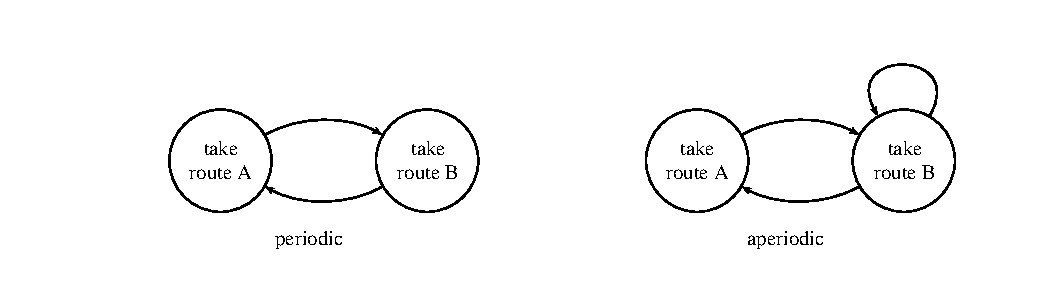
\includegraphics[width=0.99\textwidth, angle=0]{understanding/figures/mc/fig1.pdf}}%
{}
% ----------

% ----------
\createfigure%
{Example of (ir)reducibility}%
{Example of (ir)reducibility}%
{\label{fig:Example-of-(ir)reducibility}}%
{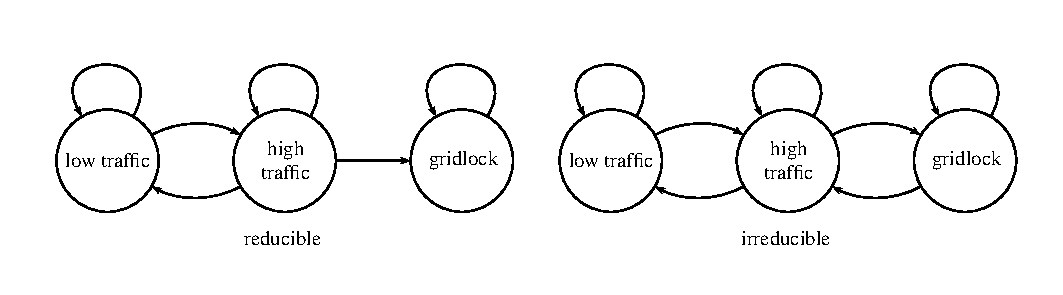
\includegraphics[width=0.99\textwidth, angle=0]{understanding/figures/mc/fig2.pdf}}%
{}
% ----------

Two key properties are aperiodicity and irreducibility. Informally,
a Markov chain is aperiodic if all of its states can be visited at
irregular times; Figure~(\ref{fig:Example-of-(a)periodicity}) provides
an example. It is irreducible if it can reach from any given initial
state any other state with one or more transitions; see Figure~(\ref{fig:Example-of-(ir)reducibility})
for an example. Aperiodicity and irreducibility are essential when
it comes to long-term predictions, where (i) aperiodicity guarantees
that the concrete iteration at which one evaluates the simulation
does not play a role and (ii) irreducibility ensures that every possible
future system state can be reached (predicted) by the simulation.
If both properties are given, the Markov chain has the following properties
\citep{ross-2006}:
\begin{enumerate}
\item A unique stationary distribution exists. The simulation process attains
this distribution after {}``many'' iterations, independently of
its initial state.
\item It is feasible to compute statistics of the stationary distribution
from a single simulation run, meaning that it is not necessary to
run replications.
\label{it:self-averaging}
\end{enumerate}

With respect to \gls{matsim}, the following holds: %\kai{@Gunnar: Das habe ich
% aufgrund unsere Diskussionen neu versucht; schaust Du es bitte durch?  Danke.}
\begin{itemize}

\item Periodicity is already broken if there exists a nonzero probability of staying in
the same state. This is possible in MATSim 
%if agents have a finite memory
because the following sequence of events may occur by chance:
%% as often as the agent memory is long: 
(i) no agent uses plan innovation,
(ii) all agents select the same plan as in the previous iteration, 
(iii) the mobility simulation creates identical congestion and travel time patterns 
%% as in the previous iteration.
such that $Z^k$ from \MyEqRef{eq:learning-model} remains the same as $Z^{k-1}$; practically, this means that all plan scores remain the same. 
%% \kai{@Gunnar: Habe das mal umgeschrieben, weil in der praktischen Implementierung die Agenten kein Memory haben; sie merken sich nur den geglätteten Score.}  
%% \gunnar{ok}

The above is a rather formal argument; more intuitively, the stochasticity in \gls{matsim} means that even if the system returns multiple times exactly to a state where it has been before, it is improbable that it does so with the same number of steps. 
%% \kai{@Gunnar: pls chk the above.}
%% \gunnar{ok}

%% \gunnar{Kai, Du hattest Folgendes geschrieben: ``Periodicity is easily broken by stochasticity.  
%% Given the many sources of stochasticity in MATSim, it is improbable that deterministic cycles exist.''
%% Ich finde das problematisch, weil MCs ``by design'' stochastisch sind; periodicity und stochasticity
%% schliessen einander nicht aus.} \kai{Vielleicht einfach so: das Diagramm 9.3(links) kommt in matsim sozusagen nicht vor.}

%% \kai{Mir würde es plausibel erscheinen, wenn wir das auf einen bestimmten Zustand beziehen.  Wenn wir davon ausgehen, dass Innovation ausgeschaltet ist, dann fällt (i) weg.  Danach bleibt dann die Frage, was ein ``state'' ist; wenn dies der Vektor der gewählten Pläne ist, dann reicht (ii) bereits aus für ``staying in same state''.  Wenn die ``plan scores'' zu ``state'' dazu gehören, dann brauchen wir auch noch, dass die scores bereits konvergiert sind.}

\item With plan innovation (see Sections~\ref{sec:strategymodules}, \ref{sec:innovation-switchoff} and~\ref{sec:innovation}) switched on, the system is in general not irreducible:
%% The MATSim property that causes problems when it comes to irreducibility are the changes to the set of possible plans per agent: 
Every time a new plan is added somewhere, the previous subspace of the state space where the plan was not available \emph{cannot} be reached any more until that plan is removed; similarly, every time a plan is removed, the previous subspace of the state space where the plan was available cannot be reached any more until the plan is re-created again. (Chapter~\ref{ch:discretechoice} discusses this in greater detail and also suggests a cure to this problem.)

Even if plans creation and removal could be modelled such that irreducibility was guaranteed, the dynamics of this process would, due to the size of the state space, be slow.

 %% that it would be impractial to sample over the resulting iterations. Thus, although the above item~\ref{it:self-averaging} would be formally correct, one would never have enough iterations to put it to practical use.  \gunnar{Sind wir da sicher? Wenn wir uns nur f\"ur niedrigdimensionale projections interessieren, dann mag es durchaus sein, dass sich diese projections hinreichend schnell durchmischen. Ich bin zumindest nicht daf\"ur, die M\"oglichkeit von vorneherein auszuschliessen.}


\item With plan innovation switched off, 
MATSim in its {}``standard configuration'' is likely to 
% have
%% these properties if the plan choice sets of all agents are a priori
%% defined, meaning technically that all {}``plan innovation'' modules
%% are switched off and that only {}``plan selection'' modules are
%% used. 
be irreducible.  This is only {}``likely'' because the notion of a {}``standard
configuration'' itself is not rigorously specified here. The arguments
behind this follow \citet{cascetta-1989}, who presents a related
result for a much simpler, trip-based traffic simulation that only
allows for route choice. Observing that travel plans are, technically,
paths in a rather complicated decision network then allows to carry
this result over to MATSim. See also \citet{NagelEtc2000tristan-succ} and \citep{floetteroed-2010e}.

%% \kai{@Gunnar: Du erwähnst in Deiner Email etwas von ``finite score memories''.  Kann leider nicht sagen, wie sich das überträgt: matsim in std config hat eigentlich gar kein memory.  Von vorherigen Iterationen übrig bleiben nur die scores, die evtl.\ auch noch gemittelt sind.  Es kann allerdings sein, dass es sehr lange her ist, dass ein Plan zum letzten Mal angefasst wurde, und der Score daher sehr alt ist.

%% Normalerweise ist es damit erledigt, denn das mit dem ``finite memory'' hat, so wie ich es kenne, eigentlich nur etwas mit dem ``finite state space'' zu tun.

%% Außerdem hat (normalerweise) jeder Plan in jeder Iteration eine non-zero proba, gewählt zu werden, m.E.\ eine weitere Versicherung gegen ``Probleme''.
%% }

%% \gunnar{ok. Das ist jetzt ja auch so vorsichtig formuliert, dass es eigentlich gar nicht falsch sein kann.}

\item In the particular case of the scores being additionally forced to their 
expected values (Section~\ref{sec:score-msa}), the system eventually draws
agent behavior from fixed choice distributions and hence varies independently
from one iteration to the next.

In the case the config option \lstinline|ChangeExpBeta| is used, some
correlation is maintained between the choices in subsequent iterations, 
even though the long-term choice distributions remain unchanged.

\end{itemize}

% MATSim with variable plan choice sets, is unlikely to have these properties,
% at least if the currently used {}``plan innovation'' modules are
% used. The reason for this is that plan innovation is at least in parts
% based on best response behavior, which may limit behavioral variability
% to the extent that irreducibility is destroyed. (Chapter~\ref{ch:discretechoice}
% discusses this in greater detail and also suggests a cure to this
% problem.) This means, that MATSim with plan innovation turned on (i)
% may yield different simulation results depending on how the simulation
% process is initialized (empirical evidence for this is indicated in
% Chapter~\note{REF: Kai mentioned this in the past; is it documented somewhere?} 

% \kai{Nein, eigentlich hatten wir das nie.  Effekte, an die ich mich erinnern kann 
% (nicht notwendigerweise verbunden mit obiger Aussage), sind:
% \begin{itemize}
% %
% \item Wenn man den scale parameter zu groß macht (also stark deterministische best response Reaktion) 
% \emph{und} TimeMutation verwendet, dann kann es Periodizitäten geben \citep{RaneyNagel2006traf-framework}. 
% -- Ich habe immer spekuliert, dass das reine route assignment problem auch bei uns die 
% Stabilitätseigenschaften von static asssignment irgendwie erbt.
% %
% \item Network breakdowns \emph{in aufeinanderfolgenden Iterationen} kommen vor allem aus der 
% (best reply) innovation. Wenn man Innovation abschaltet, verschwinden sie ganz; wenn man die Mobsim 
% mit immer den gleichen Plänen startet, verschwinden sie \emph{nicht}, sind aber nicht 
% mehr über die Iterationen korreliert (was ja auch kein Wunder ist).  
% Siehe \citep{RieserNagel2008NetworkBreakdown}. -- Leider sagt das Paper nicht genau, 
% ob es mit \lstinline{ChangeExpBeta} oder mit \lstinline{SelectExpBeta} gerechnet wurde. :--(
% %
% \item Die network breakdowns verschwinden auch, wenn man die storage capacity auf den Kanten hochdreht.  
% Das kam mal von David Charypar, aber der hat das leider nie aufgeschrieben.  
% Hat was damit zu tun, dass bei hoher storage capacity die queue, die nötig ist, um eine schnelle Kante 
% mit einer langsameren zu balancieren, dann in die Kante selber reinpasst, damit keinen spill-back mehr 
% bildet, und damit keinen network breakdown mehr auslöst.
% \end{itemize}
% %
% })
% and that (ii) statistics of interest cannot be obtained from a single
% MATSim run.

% \note{Mention broken ergodicity?}

In summary, there exists a mathematical framework that allows to somewhat
rigorously characterize the outcome of MATSim's relaxation process.
It turns out that MATSim in its current form is not necessarily a ``well-behaved''
stochastic process, but casting it into this framework also enables a structured
approach of developing the simulation logic further. An example of how to go
about this is given Chapter~\ref{ch:discretechoice}.


%\gunnar{Ich habe die ``breakdown''-Diskussion jetzt rausgenommen; alles was ich da ausprobiert habe, war zu
%technische und konstruiert, als dass es dem Kapitel weiterhelfen w\"urde.}


%\subsection{Reducing variability \textcolor{gray}{Avoiding Network Breakdowns}}

% \subsection{The effect of (implicitly) synchronized agent behavior}
% 
% % \kai{Vermeidet nicht network breakdown (siehe Zusammenfassung oben) ... 
% % bzw.\ es ist zumindestens unklar.  Meiner Erinnerung nach hatte ich \lstinline{ChangeExpBeta} 
% % eingeführt, weil das equil net scenario sehr schlecht konvergierte.  Und das ist ja auch klar: 
% % Wenn $N$ Agenten die selben zwei gleich gute Optionen haben, dann ist die Amplitude der 
% % Fluktuationen auf einer Option $\sim \sqrt{N}$.  -- Ob das allerdings so funktioniert wie gedacht, 
% % weiß ich nicht.  Wenn man die scores zum Konvergieren bringt, kann es ja keinen Unterschied 
% % mehr machen.  Also muss es, wenn überhaupt, etwas damit zu tun haben, dass die scores nur 
% % die letzte Planausführung reflektieren. -- Aber da das mit der switching proba auch einfacher 
% % und eleganter ist, bin ich dabei geblieben. } 
% 
% % \kai{Ich habe hier irgendwie kein gutes Gefühl bei.  ERSTENS ist unklar, ob es wirklich
% %  mit dem network breakdown etwas zu tun hat.  Da kannst Du jetzt schimpfen, dass wir das 
% %  unsauber aufgeschrieben haben, aber es hilft nichts.  ZWEITENS kann es ja nicht sein, dass wir 
% %  die gleiche stationäre Verteilung bekommen, aber eine geringere breakdown proba.  
% %  Ich denke auch, dass wir dann doch eine andere Verteilung der $Z$ bekommen.  Aber ich habe keine 
% %  Intuition, was das bzgl.\ breakdown tut ... z.B.\ könnte das System auch einfach mehr 
% %  Iterationen brauchen, um sich an den kritischen Zustand heranzutasten, und dann dauert die 
% %  ``Lawine'' auch länger, um davon wieder wegzukommen.  (Dann würde sich wohl das $Z^{crit}$ verändern.)}
% 
% % \kai{Irgendwie müssen wir dringend mal einen Antrag schreiben, der diese Dynamiken untersucht, 
% % und dafür jemanden einstellen, den das interessiert.  Derzeit habe ich die Situation, dass das sogar 
% % aus Anträgen immer wieder rausfliegt, weil keiner außer mir die entsprechenden work packages schreiben kann.}
% 
% 
% Section~\ref{sec:ag-based-assignment-selection}presents the \texttt{ExpBetaPlanChanger}
% as an alternative to the \texttt{ExpBetaPlanSelector} that offers (i) better convergence
% properties (smoother transients) and (ii) identical stationary plan choice distributions 
% at the individual-agent level. 
% 
% System modifications that exclusively affect the transients are uncritical from the modeling
% perspective, which is exclusively concerned with the simulation behavior in stationary
% conditions. In this regard, the \texttt{ExpBetaPlanChanger} is nothing but a computationally
% advantageous simulation scheme. 
% 
% The following presentations deploys the MC perspective on MATSim in order to analyze
% the effect of using the \texttt{ExpBetaPlanChanger} on the stationary behavior of the
% simulation as a whole -- which turns out to be potentially different from the stationary 
% behavior of a set of independent agents.
% 
% % \kai{Kann es (natürlich) nur, wenn es eben doch nicht das gleiche stationäre Modell ist.}
% 
% \gunnar{(to self) Continue here.}
% 
% To keep the presentation tractable, it is assumed that a network breakdown
% occurs if and only if a sufficiently large number of agents selects
% a {}``critical travel plan''. It further is assumed that the probability
% of selecting a critical plan is zero unless a {}``critical path''
% of events has occurred in the past. The recent occurrence of such
% a path is instantaneously reflected by the system being in a {}``critical
% state''. Formally, the probability of a breakdown given that the
% system is in a critical state can be written as
% \begin{eqnarray}
% P(\text{breakdown}\mid Z^{\text{crit}}) & = & P\left(\left[\frac{1}{N}\sum_{n=1}^{N}\mathbf{1}(i_{n}\in C_{n}^{\text{crit}}\mid Z^{\text{crit}})\right]\geq\phi^{\text{crit}}\right)
% \end{eqnarray}
% \kai{habe da noch eine weitere Klammer reingebaut}
% where $Z^{\text{crit}}$ is the event of the system being in a critical
% state, $C_{n}^{\text{crit}}$ is the set of critical plans of agent
% $n$ and $\mathbf{1}(i_{n}\in C_{n}^{\text{crit}}\mid Z^{\text{crit}})$
% indicates if agent $n$ selects a critical plan $i_{n}$ given that
% the system is currently in a critical state. Letting $N$ be the total
% number of agents, then $\frac{1}{N}\sum_{n=1}^{N}\mathbf{1}(\cdot)$ represents
% the fraction of agents selecting a critical plan. The breakdown probability
% is then given by the probability that this fraction is larger than
% a critical value $\phi^{\text{crit}}$. As $N$ gets larger, the variance
% of the average value $\frac{1}{N}\sum_{n=1}^{N}(\cdot)$ gets smaller.
% This means that for a large agent population it is reasonable to approximate
% this quantity by its expectation. Observing further that $\text{E}\{\mathbf{1}(\text{event }X\text{ happens})\}=P(X)$,
% one obtains
% \begin{eqnarray}
% P(\text{breakdown}\mid Z^{\text{crit}}) & \approx & \mathbf{1}\left(\frac{1}{N}\sum_{n=1}^{N}P(i_{n}\in C_{n}^{\text{crit}}\mid Z^{\text{crit}})\geq\phi^{\text{crit}}\right),\label{eq:breakdown-indicator}
% \end{eqnarray}
% meaning that if the system is currently in a critical state then a
% breakdown is guaranteed if and only if the average probability of
% selecting a critical plan over all agents in the population exceeds
% $\phi^{\text{crit}}$.
% 
% Denote the probability that agent $n$ selects plan $i$ given the
% information $Z$ by $P_{n}(i\mid Z)$. Assume that this choice distribution
% can lead to breakdowns. Now consider a modification of the plan choice
% mechanism that selects, for each agent, with probability $\alpha$
% a plan according to $P_{n}(i\mid Z)$ and otherwise according to $P_{n}(i\mid\tilde{Z})$,
% with $\tilde{Z}$ being the simulator state (information) from a randomly
% selected previous iteration. Assuming stationarity, this yields
% \begin{eqnarray}
% \tilde{P}_{n}(i\mid Z) & = & \alpha P_{n}(i\mid Z)+(1-\alpha)\sum_{\tilde{Z}}P_{n}(i\mid\tilde{Z})\Pi(\tilde{Z})\label{eq:modifed-choice}
% \end{eqnarray}
% with $\Pi(\tilde{Z})$ being the stationary distribution of the simulator
% states. This resembles the \texttt{ExpBetaPlanChanger} in the sense
% that past iterations are recycled: Here, this happens by using past
% information whereas the \texttt{ExpBetaPlanChanger} realizes a similar
% effect by increasing the number of iterations during a previously
% selected plan is maintained. Another similarity is that (\ref{eq:modifed-choice})
% does, just like the \texttt{ExpBetaPlanChanger}, not change the agent's
% stationary choice distribution:
% \begin{eqnarray}
% \tilde{\Pi}_{n}(i) & = & \sum_{Z}\tilde{P}_{n}(i\mid Z)\Pi(Z)\\
%  & = & \sum_{Z}\left[\alpha P_{n}(i\mid Z)+(1-\alpha)\sum_{\tilde{Z}}\alpha P_{n}(i\mid\tilde{Z})\Pi(\tilde{Z})\right]\Pi(Z)\\
%  & = & \alpha\sum_{Z}P_{n}(i\mid Z)\Pi(Z)+(1-\alpha)\sum_{\tilde{Z}}P_{n}(i\mid\tilde{Z})\Pi(\tilde{Z})\sum_{Z}\Pi(Z)\\
%  & = & \sum_{Z}P_{n}(i\mid Z)\Pi(Z).
% \end{eqnarray}
% 
% 
% Now the effect of inserting this model into the simulation as a whole
% is considered. For this, recall that $P_{n}(i_{n}\in C_{n}^{\text{crit}}\mid Z)$
% is nonzero only for $Z=Z^{\text{crit}}$, implying
% \begin{eqnarray}
% \tilde{P}_{n}(i_{n}\in C_{n}^{\text{crit}}\mid Z^{\text{crit}}) & = & \alpha P_{n}(i_{n}\in C_{n}^{\text{crit}}\mid Z^{\text{crit}})+(1-\alpha)\sum_{\tilde{Z}}P_{n}(i_{n}\in C_{n}^{\text{crit}}\mid\tilde{Z})\Pi(\tilde{Z})\\
%  & = & \alpha P_{n}(i_{n}\in C_{n}^{\text{crit}}\mid Z^{\text{crit}})+(1-\alpha)P_{n}(i_{n}\in C_{n}^{\text{crit}}\mid Z^{\text{crit}})\Pi(Z^{\text{crit}})\\
%  & = & [\alpha+(1-\alpha)\Pi(Z^{\text{crit}})]P_{n}(i_{n}\in C_{n}^{\text{crit}}\mid Z^{\text{crit}}).
% \end{eqnarray}
% Inserting this into (\ref{eq:breakdown-indicator}) results in the
% modified breakdown probability
% \begin{eqnarray}
% \tilde{P}(\text{breakdown}\mid Z^{\text{crit}}) & \approx & \mathbf{1}\left(\frac{1}{N}\sum_{n=1}^{N}\tilde{P}(i_{n}\in C_{n}^{\text{crit}}\mid Z^{\text{crit}})\geq\phi^{\text{crit}}\right),\\
%  & = & \mathbf{1}\left(\frac{1}{N}\sum_{n=1}^{N}P_{n}(i_{n}\in C_{n}^{\text{crit}}\mid Z^{\text{crit}})\geq\frac{\phi^{\text{crit}}}{\alpha+(1-\alpha)\Pi(Z^{\text{crit}})}\right).
% \end{eqnarray}
% This expression looks like (\ref{eq:breakdown-indicator}), only that
% the threshold value $\phi^{\text{crit}}$ is now divided by $\alpha+(1-\alpha)\Pi(Z^{\text{crit}})$.
% This denominator ranges from $\Pi(Z^{\text{crit}})$ (for $\alpha=0$)
% to one (for $\alpha=1$), meaning that the breakdown threshold is
% increased by decreasing $\alpha$.
% 
% Intuitively: For a breakdown to happen, enough agents must simultaneously
% select a critical plan. The unmodified simulation synchronizes the
% plan choices by conditioning all of them on the current system state:
% If the system can break down at all, then according to (\ref{eq:breakdown-indicator})
% it will do so once a critical state is reached. The modified plan
% choice logic breaks this synchronization, in the sense that the occurrence
% of a critical state alone is no more sufficient to trigger plan choices
% that lead to a breakdown. Additionally, enough agents must base their
% replanning on past state that was by chance also critical.
% 
% Even though this analysis does not fully represent the \texttt{ExpBetaPlanChanger}
% (which would be more involved because then further complications such
% as score difference thresholds would enter the picture), it offers
% an intuitive explanation of its stabilizing effect. The perhaps surprising
% effect of unchanged stationary choice distributions at the individual
% level leading to a change in the overall system's state can be explained
% by the different ways in which agent behavior can be synchronized.




\section{\label{sec:Statistical-analysis-of}Analyzing Simulation Outputs}

%\note{I don't know how useful this is. Perhaps move it to an earlier chapter with a more practical focus?}
%
%\kai{Würde es erstmal hier lassen.  Man kann ja drauf verweisen.  Wir können es ggf.\ immer noch später umstellen.}

Many of the models used in MATSim are stochastic, for instance random
utility models for plan choice or the randomized selection of the
next vehicle to enter a congested downstream link in the mobility
simulation. The reason for this randomness is that real mobility and
transportation processes are understood only to a limited degree.
The insertion of randomness represents the remaining uncertainty in
the modeling. 

This uncertainty may apply to both (i) model inputs, meaning that
random variables are computed once before a simulation run and then
kept fixed (for instance, the random generation of a synthetic population)
and to (ii) processes, meaning that random variables are computed
throughout the simulation (for instance, the repeated evaluation of
discrete choice models). Technically, if a MATSim scenario is simulated
$R$ times, with different random seeds, one obtains $r=1\ldots R$
independent simulation outputs $y_{r}$. Note that while the raw outputs
are plans and event files, the actual quantities for which $y_{r}$
stands here are numerical in in the majority of applications.

Given that one has used different random seeds, $y_{1},\ldots,y_{R}$
constitute independent draws from a distribution $\Pi(y)$. This means
that if one performed a huge number of simulation runs and plotted
a (possibly multidimensional) histogram of the $y$ values, then this
histogram would eventually attain the shape of $\Pi(y)$. It is important
to acknowledge that stochastic simulation outputs are a desirable
consequence of the stochasticity inserted elsewhere in the simulation:
Just as the output of a deterministic model is a truthful representation
of the consequences of its input, a stochastic model output contains
a truthful representation of the prediction uncertainty that results
from uncertainties in its input and its process specification.

To help intuition, one may think in the following of $y_{r}$ as a
large vector that contains the travel times on all links in all one-hour
time bins as observed during the last iteration of the $r$th simulation
run. Questions of the following type may then be asked:
\begin{itemize}
\item What travel times can one expect on average?
\item What is the travel time variability?
\item How probable are travel times beyond some threshold $\theta$?
\item ...
\end{itemize}
This list can be arbitrarily continued. It turns out that most (if
not all) of these questions can also be expressed symbolically. For
instance:
\begin{itemize}
\item What travel times can one expect on average?
\begin{eqnarray}
\text{E}\{y\} & = & \sum_{y}y\cdot\Pi(y)\label{eq:question-exp}
\end{eqnarray}
This asks for the expected value of the simulation output distribution.
\item What is the travel time variability?
\begin{eqnarray}
\text{VAR}\{y\} & = & \sum_{y}(y-\text{E}\{y\})^{2}\cdot\Pi(y)\label{eq:question-var}
\end{eqnarray}
This asks for the variance (or, for multidimensional outputs, the
variance-covariance matrix).
\item How probable are travel times beyond some threshold $\theta$?
\begin{eqnarray}
\text{Pr}(y\geq\theta) & = & \sum_{y}\mathbf{1}(y\geq\theta)\cdot\Pi(y)\label{eq:question-proba}
\end{eqnarray}
This expression merely sums up the probabilities of all simulation
outputs that exceed the threshold.
\item ...
\end{itemize}
This enumeration of symbols reveals a common structure. The mathematical
formulation of each question can be written in the form
\begin{equation}
\sum_{y}m(y)\cdot\Pi(y)\label{eq:exp-of-m}
\end{equation}
with different specifications of $m(y)$:

\begin{center}
\begin{table}[H]
\caption{\label{tab:Examples-of-m}Examples of $m$ functions.}


\centering{}%
\begin{tabular}{r|l}
\hline 
quantity of interest & corresponding $m(y)$ \tabularnewline
\hline 
$\text{E}\{y\}$ & $y$\tabularnewline
$\text{VAR}\{y\}$ & $(y-\text{E}\{y\})^{2}$\tabularnewline
$\text{Pr}(y\geq\theta)$ & $\mathbf{1}(y\geq\theta)$\tabularnewline
$\ldots$ & $\ldots$\tabularnewline
\hline 
\end{tabular}
\end{table}

\par\end{center}

By definition, \MyEqRef{eq:exp-of-m} is the expectation $\text{E}\{m(y)\}$
given that $y$ is distributed according to its stationary distribution
$\Pi(y)$. Combining this with the observation that the mean over
a sample converges to its expectation as the number of samples grows
(the Law of Large Numbers), one obtains
\begin{eqnarray}
\text{E}\{m(y)\} & = & \sum_{y}m(y)\cdot\Pi(y)\label{eq:define-question}\\
 & = & \lim_{R\rightarrow\infty}\frac{1}{R}\sum_{r=1}^{R}m(y_{r})\\
 & \approx & \frac{1}{R}\sum_{r=1}^{R}m(y_{r})\qquad\text{for a finite }R,\label{eq:approximate-answer}
\end{eqnarray}
where the simulation outputs $y_{r}$, $r=1\ldots R$, are independent
draws from $\Pi(y)$.

Now recall the original problem of asking certain questions about
the simulation outputs. The first row \MyEqRef{eq:define-question}
represents exactly these questions in a formal way -- and the last
row \MyEqRef{eq:approximate-answer} provides a simple recipe to compute
the answers of these questions, which reads as follows:
\begin{enumerate}
\item Define the function $m(y)$ that represents the question of interest.
\item Perform $R$ independent simulation runs and obtain the outputs $y_{1},\ldots,y_{R}$.
\item Compute $m(y_{r})$ for all $r=1\ldots R$ and average these numbers.
\end{enumerate}
Returning to the example questions, one hence obtains the following:
\begin{itemize}
\item What travel times can one expect on average?
\begin{eqnarray}
\text{E}\{y\} & \approx & \frac{1}{R}\sum_{r=1}^{R}y_{r}
\end{eqnarray}
Not surprisingly, this turns out to be the mean value over all simulated
travel times.
\item What is the travel time variability?
\begin{eqnarray}
\text{VAR}\{y\} & \approx & \frac{1}{R}\sum_{r=1}^{R}(y_{r}-\text{E}\{y\})^{2}
\end{eqnarray}
This is the empirical variance of the simulated travel times. (Note
that in practice $\text{E}\{y\}$ needs to be replaced by its estimator.)
\item How probable are travel times beyond some threshold $\theta$?
\begin{eqnarray}
\text{Pr}(y\geq\theta) & \approx & \frac{1}{R}\sum_{r=1}^{R}\mathbf{1}(y_{r}\geq\theta)
\end{eqnarray}
This divides the number of times the threshold was exceeded by the
total number of experiments, i.e.\ it yields the frequency of the event
of interest.
\item ...
\end{itemize}
Revisiting Section~\ref{sec:Existence-and-uniqueness}, it may
be possible to make these computations more efficient. If (i) there
is no uncertainty in the model inputs and (ii) the simulation uses
fixed choice sets, then its likely to be feasible to compute the above
statistics by averaging over many stationary iterations of a single
simulation run instead of having to run a large number of replications
to convergence. 

Practically, all of this is just a starting point. Important questions,
such as how precise these estimates are, how many runs one needs to
obtain a certain level of precision, etc. are not answered here; 
\citet{ross-2006} is a good starting point for further reading. 


\section{\label{sec:Summary}Summary}

This chapter attempted to clarify certain mechanisms underlying MATSim's
iterative solution scheme. The specification of MATSim's model (components)
was distinguished from MATSim's iterative solution algorithm. It was
stressed that the behavioral day-to-day interpretation of MATSim is
not to be taken literally: realism can only be expected from the long-term
behavior of the process.

This long-term behavior was then related to properties of the iteration
logic using the the Markov chain formalism. MATSim was phrased as
such a chain, with its state space being comprised of the information
available for replanning. This representation was exploited to
observe that the long-term distribution of MATSim is likely to exist
and be unique if the plan choice sets are a priori fixed.
% ; and to (ii)
% provide insights into how the \texttt{ExpBetaPlanChanger} avoids network
% breakdowns. 

It further was explained that (i) there are good reasons for the stochasticity
both in MATSim's inputs and outputs; and that (ii) instead of avoiding
stochasticity where it constitutes a truthful representation of uncertainty
one should access adequate statistical techniques to make sense of
it. 

% Local Variables:
% mode: latex
% mode: reftex
% mode: visual-line
% TeX-master: "../main"
% comment-padding: 1
% fill-column: 9999
% End: 
